%----------------------------------------------------------------------------------------
%	CAPÍTULO 3
%----------------------------------------------------------------------------------------
\chapterimage{chapter_head_2.pdf} % Imagen del capítulo

\chapter{¿Cómo funciona un ordenador?}

\section{¿Qué es un ordenador?}

\section{Estructura de un ordenador}

\begin{figure}[h]
\centering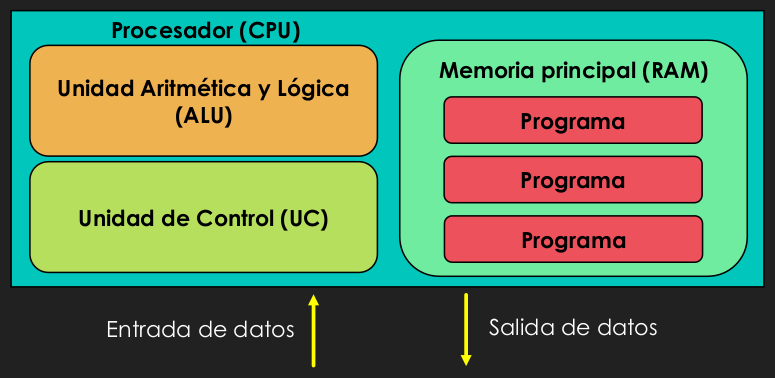
\includegraphics[scale=0.5]{estructura-ordenador1.png}
\caption{Diagrama de un ordenador}
\label{fig:c1fig1}
\end{figure}

\begin{figure}[h]
\centering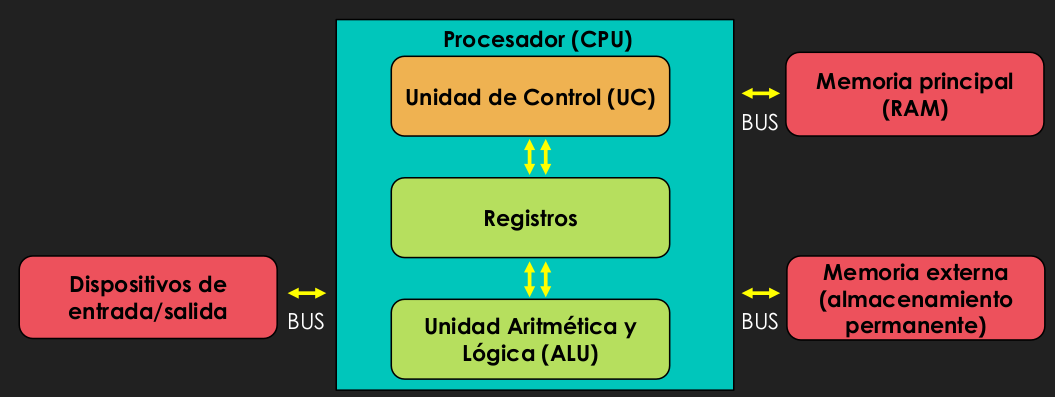
\includegraphics[scale=0.4]{estructura-ordenador2.png}
\caption{Esquema de la CPU y los buses del sistema}
\label{fig:c1fig2} 
\end{figure}

\begin{table}[h]
\centering
\begin{tabular}{l l l}
\toprule
\textbf{Unidad} & \textbf{Equivalencia}\\
\midrule
Byte (B) & 8 bits \\
Kilobyte (KB) & 1024 bytes \\
Megabyte (MB) & 1024 Kbytes \\
Gigabyte (GB) & 1024 Mbytes \\
Terabyte (TB) & 1024 Gbytes \\
Petabyte (PB) & 1024 Tbytes \\
\bottomrule
\end{tabular}
\caption{Unidades de medida de almacenamiento}
\label{tab:c1tab1} 
\end{table}

1 TB = 1024 GB = 1024 x 1024 Mb = 1.048.576 KB = 1.073.741.824 Bytes

\section{Representación de la información}

texto de prueba


\section{Ejercicios propuestos}

Completa tu aprendizaje realizando los siguientes ejercicios propuestos:

